% "{'classe':('PSI'),'chapitre':'stat_pds_2d','type':('td'),'titre':'Dépose de bagage automatique dans les aéroports', 'source':'Concours Centrale Supelec TSI 2013','comp':('B2-14','C1-05','C2-07'),'corrige':True}"
%\setchapterimage{bandeau}
\chapter*{TD \arabic{cptTD} :\\ 
Dépose de bagage automatique dans les aéroports (DBA) -- \ifprof Corrigé \else Sujet \fi}
\addcontentsline{toc}{section}{TD \arabic{cptTD} : 
Dépose de bagage automatique dans les aéroports (DBA) -- \ifprof Corrigé \else Sujet \fi}

\iflivret \stepcounter{cptTD} \else
\ifprof  \stepcounter{cptTD} \else \fi
\fi

\setcounter{question}{0}
\marginnote{Concours Centrale Supelec TSI 2013.}
\marginnote{
\UPSTIcompetence[2]{B2-14}
\UPSTIcompetence[2]{C1-05}
\UPSTIcompetence[2]{C2-07}
}

\begin{marginfigure}
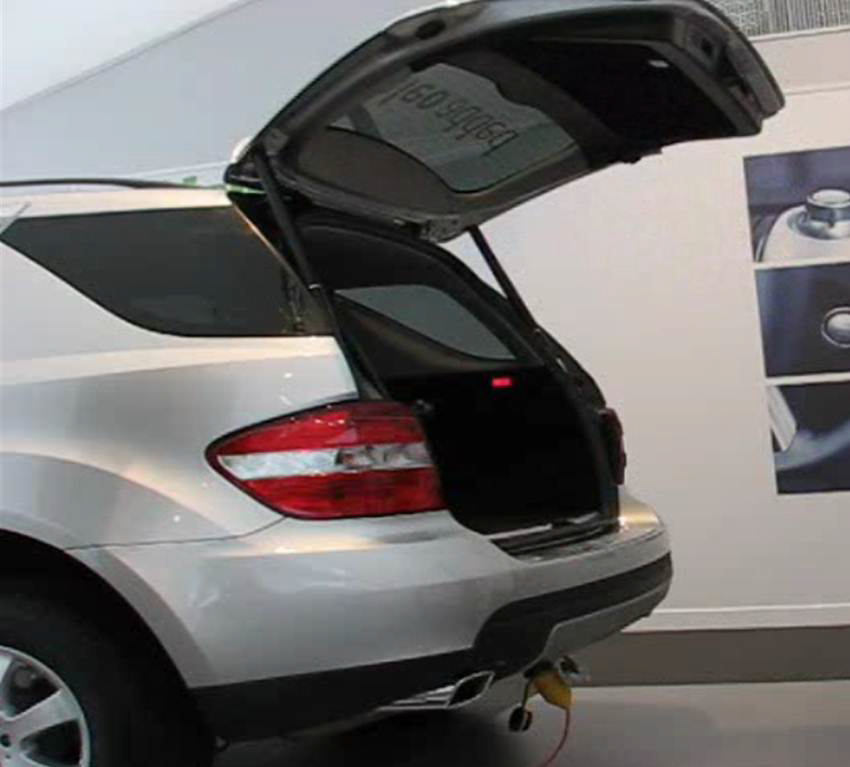
\includegraphics[width=\linewidth]{fig_00}
\end{marginfigure}



\section*{Mise en situation}
\ifprof
\else
\fi

\ifprof
\else
Le processus d’enregistrement des passagers dans les aéroports est en train de
vivre une mutation en évoluant de la « banque d’enregistrement » classique vers une idée de « dépose bagages »
automatisée. Cette évolution a été justifiée pour fluidifier le trafic passager notamment sur les destinations avec
des fréquences très importantes, par exemple certains vols Paris-Province.


Le système DBA est constitué par un basculeur actionné par un dispositif bielle-manivelle et une machine
asynchrone.


\begin{center}
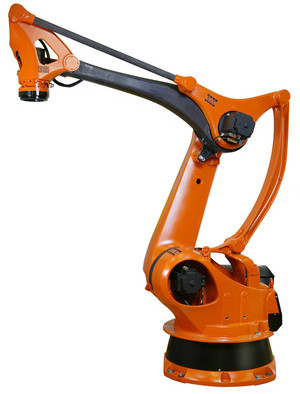
\includegraphics[width=\linewidth]{fig_01}
%\textit{}
\end{center}

\fi

\subsection*{Recherche de la vitesse de rotation maximale}
\begin{obj} 
Le bagage et le chariot sont animés par un dispositif bielle-manivelle et une machine asynchrone
triphasée avec un réducteur entraînant la manivelle. L’objectif est de déterminer la vitesse de rotation
maximale de la machine asynchrone triphasée actionnant le basculeur en accord avec l’exigence 1.4
(le basculement du bagage doit se faire en \SI{8}{s}).
\end{obj}

\ifprof
\else
Pour dimensionner correctement la machine asynchrone, la première étape est le calcul de la vitesse maximale
de l’arbre moteur.
On choisit comme loi de mouvement de rotation du moteur une loi en trapèze. On donne ainsi le profil de vitesse de rotation $\omega_r$ de l’arbre de sortie du réducteur par rapport au bâti.

\begin{marginfigure}
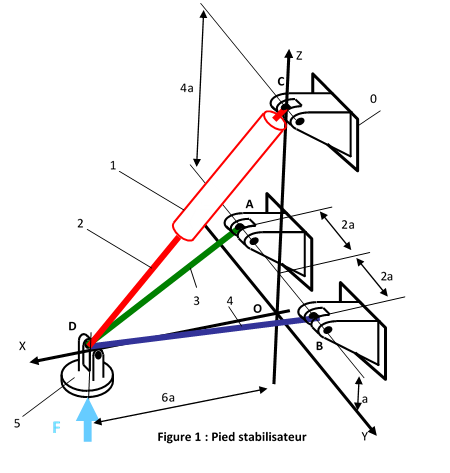
\includegraphics[width=\linewidth]{fig_02}
%\textit{}
\end{marginfigure}

Le rapport de réduction entre l’arbre moteur de vitesse de rotation et l’arbre de sortie de réducteur est noté $k=\dfrac{\omega_r}{\omega_{\text{mot}}} = \dfrac{1}{107,7}$.
Compte tenu du temps de basculement du bagage de \SI{8}{s}, les valeurs des temps sont les suivantes : $t_1=\SI{0,5}{s}$, $t_2=\SI{2,5}{s}$, $t_3=\SI{3}{s}$, $t_4=\SI{5}{s}$, $t_5=\SI{5,5}{s}$, $t_6=\SI{7,5}{s}$, $t_7=\SI{8}{s}$. L’arbre de sortie du motoréducteur doit faire un demi-tour entre 0 et $t_3$, puis un demi-tour entre $t_4$ et $t_7$.

\fi

\question{Déterminer $\omega_{\text{max}}$ en fonction des différents 
$t_i$. Faire l’application numérique.}
\ifprof
\begin{corrige}
En calculant l'aire sous la courbe (l'intégrale de la vitesse est la position) et sachant que le réducteur doit faire un demi-tour ($\pi$ rad), on a : 
$\pi = \dfrac{1}{2}t_1 \omega_{\text{max}} +\dfrac{1}{2}\left( t_3 - t_2\right) \omega_{\text{max}} + \left( t_2 - t_1\right)\omega_{\text{max}}= \left(\dfrac{1}{2}t_1  +\dfrac{1}{2}\left( t_3 - t_2\right)  + \left( t_2 - t_1\right)\right)\omega_{\text{max}} $.  On a donc $\omega_{\text{max}}  = \dfrac{\pi}{ -\dfrac{1}{2}t_1 +\dfrac{1}{2}t_2 +  \dfrac{1}{2}t_3  }=\dfrac{\pi}{ -\dfrac{1}{2}0,5 +\dfrac{1}{2}2,5  +\dfrac{1}{2} 3 }=\dfrac{\pi}{2,5}=\SI{1,26}{rad.s^{-1}}$.
\end{corrige}
\else
\fi


\question{En déduire la vitesse de rotation de l’arbre moteur maximale $\omega_{\text{mot max}}$. Faire l’application numérique et donner le résultat en $\text{tr}\cdot\text{min}^{-1}$.}

\ifprof
\begin{corrige}
$\omega_{\text{mot max}}=107,7\times 1,26 = \SI{135}{rad.s^{-1}}=\SI{1292}{tr.min^{-1}}$.
\end{corrige}
\else
\fi

\subsection*{Recherche du couple moteur maximal en vue du dimensionnement de la machine asynchrone}

\begin{obj}
La seconde étape du dimensionnement consiste à rechercher le couple moteur maximal en accord avec
l’exigence 1.2 (la masse du bagage pouvant être manœuvré par le système est de \SI{50}{kg}).
\end{obj}

%\includegraphics[width=.8\linewidth]{fig_01_bis}
%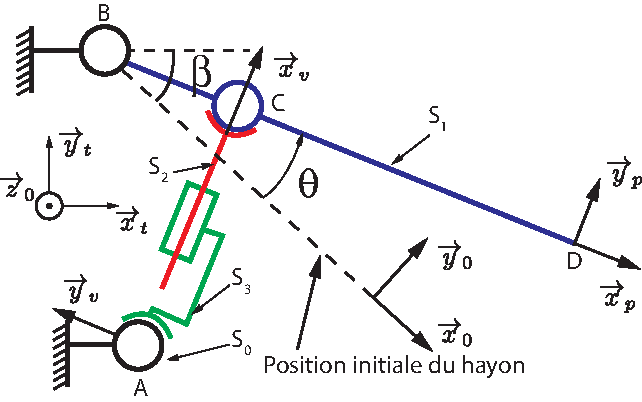
\includegraphics[width=.8\linewidth]{hayon_parametrage}
%\textit{}

\ifprof
\else


Pour calculer le couple moteur maximal, on se place dans un cas quasi-statique et on néglige tous les effets
dynamiques. Compte tenu de la construction du mécanisme (non linéaire), le couple moteur est variable et on
le calcule dans une position particulière correspondant au couple maximal.

On note :
\begin{itemize}
\item $S_0$ le bâti ;
\item $S_1$ l’ensemble constitué par le chariot, le bagage et les galets, dont le centre de gravité est noté $G$ et la masse est notée $m=\SI{80}{kg}$;
\item $S_2$ la bielle $DB$ de direction $\vect{x_2}$;
\item $S_3$ l’arbre de sortie de réducteur et la manivelle $\vect{ED}=R\vect{x_3}$ avec $R=\SI{86}{mm}$.
\end{itemize}
Le mouvement est considéré comme plan. On néglige toutes les masses sauf celle de l’ensemble $S_1$. Toutes les liaisons sont parfaites. Le référentiel lié au solide $S_0$ est considéré galiléen. On note l’accélération de la pesanteur $\vect{g}=-g\vect{y_0}$ avec $g=\SI{9,81}{m.s^{-2}}$.

Les liaisons entre $S_0$ et $S_1$ sont des liaisons sphère-plan de normales $\axe{A_1}{{x}_{11}}$ et $\axe{A_2}{{x}_{12}}$.
On note $I$ le point d’intersection des normales $\axe{A_1}{{x}_{11}}$ et $\axe{A_2}{{x}_{12}}$. On note $\vect{IB}=L_2\vect{x_{12}}$ et $\vect{IG}=x_G\vect{x_{0}}+y_G\vect{y_{0}}$.

\begin{marginfigure}
\centering
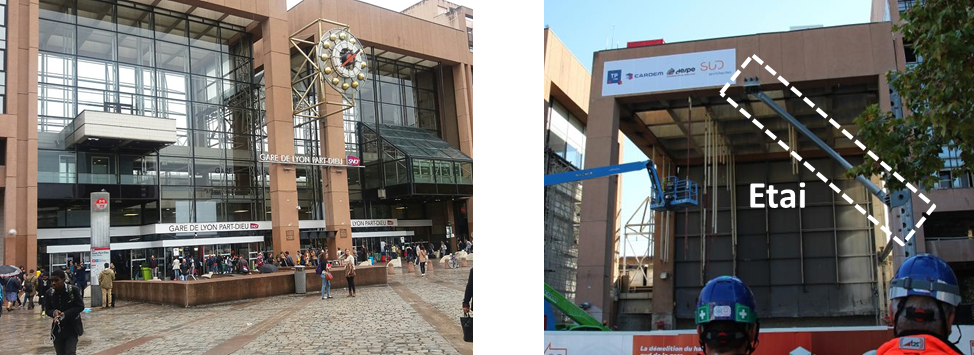
\includegraphics[width=.8\linewidth]{fig_03}
%\textit{}
\end{marginfigure}

On note les angles $\alpha_i$ formés entre les vecteurs $\vect{x}_0$ et $\vect{x}_i$: $\alpha_i=\angl{{x}_0}{{x}_i}$ avec $i\in \{2;3;11;12\}$ .



La liaison entre $S_1$ et $S_2$ est une liaison pivot d’axe $\axe{B}{z_0}$.

La liaison entre $S_2$ et $S_3$ est une liaison pivot d’axe $\axe{D}{z_0}$.

La liaison entre $S_0$ et $S_3$ est une liaison pivot d’axe $\axe{Es}{z_0}$.

\ifnormal
\else
On note $F_B$ la norme de la résultante du torseur $\torseurstat{T}{S_2}{S_1}$. 
\fi

\begin{marginfigure}
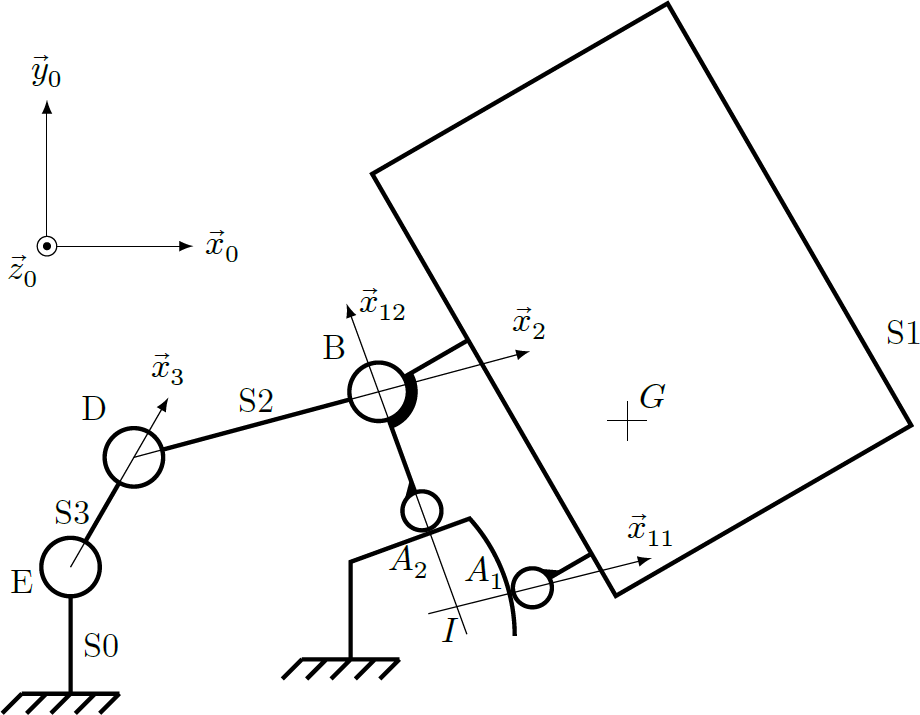
\includegraphics[width=\linewidth]{fig_04}
%\textit{}
\end{marginfigure}
\fi


\ifnormal
\question{Déterminer la forme des torseurs $\torseurstat{T}{S_0}{S_1}_1$ au point $A_1$ et $\torseurstat{T}{S_0}{S_1}_2$ au point $A_2$ des actions mécaniques des rampes du bâti $S_0$ s’appliquant sur le chariot $S_1$. Ces torseurs sont-ils des glisseurs ?}
\else
\fi


\ifprof
\begin{corrige}
$\torseurstat{T}{S_0}{S_1}_1=\torseurl{F_1\vect{x_{11}}}{\vect{0}}{A_1}$
et 
$\torseurstat{T}{S_0}{S_1}_2=\torseurl{F_2\vect{x_{12}}}{\vect{0}}{A_2}$. 
Ces torseurs sont des glisseurs (il existe un point où le moment est nul, ici les droites $(A_i,I)$). 
\end{corrige}
\else
\fi

\ifnormal
\question{La somme des torseurs $\torseurstat{T}{S_0}{S_1}_1$ et $\torseurstat{T}{S_0}{S_1}_2$ est-elle un glisseur ? Si oui, déterminer un point de son support.}
\else
\fi

\ifprof
\begin{corrige}
On a $\torseurstat{T}{S_0}{S_1}=\torseurstat{T}{S_0}{S_1}_1+\torseurstat{T}{S_0}{S_1}_2=\torseurl{F_1\vect{x_{11}}+F_2\vect{x_{12}}}{\vect{0}}{I}$. Ce torseur est un glisseur dont le point $I$ appartient au support. 
\end{corrige}
\else
\fi

\ifnormal
\question{Déterminer la forme du torseur $\torseurstat{T}{S_2}{S_1}$ de l’action mécanique de la bielle $S_2$ sur l’ensemble $S_1$ au point $B$. On notera $F_B$ la norme de la résultante de ce torseur.}
\else
\fi


\ifprof
\begin{corrige}
\textbf{On prendra $F_B$ comme valeur algébrique et pas comme norme de la résultante.}
On isole la bielle $S_2$, elle est soumise à deux glisseurs. D'après le PFS, ces glisseurs sont de même norme, de même direction  (la droite $(DB)$) et de sens opposés. 
On a $\torseurstat{T}{S_2}{S_1}=\torseurl{ F_B\vect{x_{2}}}{\vect{0}}{B}$.
\end{corrige}
\else
\fi


\ifnormal
\question{En isolant $S_1$, et en ramenant les moments en $I$, déterminer l’expression de $F_B$ en fonction de la masse $m$ de $S_1$, des angles $\alpha_i$ et des constantes du problème.}
\else
\fi

\ifprof
\begin{corrige}
On isole $S_1$. 

On réalise le BAME : 
\begin{itemize}
\item $\torseurstat{T}{S_2}{S_1}=\torseurl{ F_B\vect{x_{2}}}{\vect{0}}{B}$ 

$=\torseurl{ F_B\vect{x_{2}}}{L_2 F_B \sin  \left(\alpha_{12}-\alpha_2\right) \vect{z}}{I}$ ($\vect{IB}\wedge F_B\vect{x_{2}}=L_2\vect{x_{12}}\wedge  F_B\vect{x_{2}}$ $=L_2 F_B \sin  \left(\alpha_{12}-\alpha_2\right) \vect{z}$);
\item $\torseurstat{T}{S_0}{S_1}=\torseurl{F_1\vect{x_{11}}+F_2\vect{x_{12}}}{\vect{0}}{I}$;
\item $\torseurstat{T}{ \text{pes} }{S_1}$ $=\torseurl{-mg \vect{y_{0}}}{\vect{0}}{G}$

$=\torseurl{-mg \vect{y_{0}}}{-mgx_G\vect{z_{0}}}{I}$ ($\vect{IG}\wedge -mg \vect{y_{0}}$ $=\left(x_G\vect{x_{0}}+y_G\vect{y_{0}} \right) \wedge  -mg \vect{y_{0}}$ $= -mgx_G\vect{z_{0}}$).
\end{itemize}

En appliquant le TMS en $I$ en projection sur $\vect{z_0}$, on a : 
$L_2 F_B \sin  \left(\alpha_{12}-\alpha_2\right)  -mgx_G = 0 $ soit
$ F_B    = \dfrac{mgx_G}{L_2  \sin  \left(\alpha_{12}-\alpha_2\right)} $. 
\end{corrige}
\else
\fi

\question{On note $C_{\text{red}}$ le couple exercé par l’arbre de sortie de réducteur sur la manivelle $S_3$. Montrer que $C_{\text{red}}-RF_B \sin \left( \alpha_3 - \alpha_2\right) = 0$.}
\ifprof
\begin{corrige}
En isolant 2, on montre que $\torseurstat{T}{2}{3}=\torseurstat{T}{1}{2}$. 

On isole 3. 

On fait le BAME :
\begin{itemize}
\item $\torseurstat{T}{2}{3}=-\torseurstat{T}{2}{1}=\torseurl{ -F_B\vect{x_{2}}}{\vect{0}}{D}$ et on a $\vectm{E}{2}{3} = \vectm{D}{2}{3} + \vect{ED}\wedge -F_B\vect{x_{2}}$ $=R\vect{x_3}\wedge -F_B\vect{x_{2}}$ $=-RF_B \sin\left( \alpha_3- \alpha_2\right)$;
\item $\torseurstat{T}{\text{réd}}{3}$ $ = \torseurl{ \vect{0}}{C_{\text{red}}\vect{z_0}}{E}$;
\item $\torseurstat{T}{0}{3}$ avec $\vectm{E}{0}{3}\cdot \vect{z_0} = 0$.
\end{itemize}
On applique le TMS en $E$ en projection sur $\vect{z_0}$ : $C_{\text{red}}-RF_B \sin \left( \alpha_3 - \alpha_2\right) = 0$.
\end{corrige}
\else
\fi

Dans la configuration choisie, on a $x_G=\SI{506}{mm}$, $L_2 = \SI{140}{mm}$, $\alpha_3=91\degres$, $\alpha_{12}=108\degres$  et $\alpha_2=3\degres$ (on montre par une simulation numérique que cette position conduit au couple maximal).

\ifnormal
\question{En déduire l’expression du couple $C_{\text{red}}$ qu’exerce le réducteur sur la manivelle $S_3$ en fonction du poids du chariot, des angles $\alpha_i$ et des constantes du problème. Faire l’application numérique.}
\else
\fi

\ifprof
\begin{corrige}
On a $C_{\text{red}}=RF_B \sin \left( \alpha_3 - \alpha_2\right) =\dfrac{ Rmgx_G \sin \left( \alpha_3 - \alpha_2\right)}{L_2  \sin  \left(\alpha_{12}-\alpha_2\right)} \simeq \SI{252}{Nm}$.
\end{corrige}
\else
\fi

\question{En déduire la valeur numérique $C_m$ du couple qu’exerce l’arbre de la machine asynchrone sur l’arbre
d’entrée du réducteur (on supposera le rendement du réducteur égal à 1).}
\ifprof
\begin{corrige}
Le couple moteur est alors de \SI{2,34}{Nm}.
\end{corrige}
\else
\fi









\ifprof
\else
\ifcolle
\else
\begin{marginfigure}
\begin{solution}
\begin{enumerate}
\item \SI{1,26}{rad.s^{-1}}.
\item \SI{1292}{tr.min^{-1}}.
\item Oui.
\item $I$.
\item  $\torseurl{ F_B\vect{x_{2}}}{\vect{0}}{B}$.
\item $ F_B    = \dfrac{mgx_G}{L_2  \sin  \left(\alpha_{12}-\alpha_2\right)} $.
\item $C_{\text{red}}-RF_B \sin \left( \alpha_3 - \alpha_2\right) = 0$.
\item \SI{252}{Nm}.
\item \SI{2,34}{Nm}.
\end{enumerate}
\end{solution}
\end{marginfigure}
\fi
\fi

